\subsection{H6 -- Feature and augmentation ablation}
\label{sec:ablation}
Table~\ref{tab:ablation} retrains the 1D-CNN and the SVM on the paper-protocol split with parts of the input removed.
The test set has 144 clips, so one clip is \AblClipPct{} points and the standard error of an accuracy near 79\%
is about \AblSE{} points; differences smaller than roughly twice that are not meaningful.

\begin{table}[t]
\centering
\caption{Ablation on the paper-protocol split (accuracy \%, 144 test clips). $\Delta$ is relative to the full
1D-CNN (79.2\%). *Training stopped at epoch 9 with validation accuracy at chance level (see text).}
\label{tab:ablation}
\footnotesize\setlength{\tabcolsep}{3pt}
\resizebox{\columnwidth}{!}{\begin{tabular}{lcccc}
\toprule
Variant & Input dim. & SVM acc. & 1D-CNN acc. & $\Delta$ CNN (pp) \\
\midrule
All features (ZCR+RMSE+MFCC+Chroma) & 3{,}672 & 77.1 & 79.2 & -- \\
without ZCR & 3{,}564 & 77.1 & 79.9 & +0.7 \\
without RMSE & 3{,}564 & 77.1 & 79.2 & +0.0 \\
without MFCC & 1{,}512 & 45.1 & 56.9 & $-$22.2 \\
without Chroma & 2{,}376 & 79.2 & 73.6 & $-$5.6 \\
MFCC only & 2{,}160 & 78.5 & 80.6 & +1.4 \\
No augmentation (paper early stopping) & 3{,}672 & 78.5 & 31.2 & $-$47.9 \\
No augmentation, patience 20 & 3{,}672 & -- & 74.3 & $-$4.9 \\
\bottomrule
\end{tabular}
}
\end{table}

\begin{itemize}
  \item \textbf{MFCC is essential.} Removing the 20 MFCCs changes accuracy by \AblNomfcc{} points for the 1D-CNN and
        \AblSvmNomfcc{} for the SVM, the only feature removal clearly beyond noise. \emph{MFCC alone}
        (\AblAccMfcconly\%) is at least as accurate as the full feature set.
  \item \textbf{ZCR and RMSE add nothing measurable} ($\Delta$ of \AblNozcr{} and \AblNorms{} points).
  \item \textbf{Chroma: inconsistent.} Removing Chroma changes the 1D-CNN by \AblNochroma{} points but
        the SVM by \AblSvmNochroma{} (opposite directions). Both changes are within about two standard errors, so we find no
        robust evidence for the paper's LIME-based claim that Chroma contributes substantially.
  \item \textbf{Augmentation helps modestly, and interacts with early stopping.} Without augmentation, training
        stops at epoch 9 with validation accuracy still at chance, giving \AblAccNoaugmentation\%. The cause is that an
        un-augmented epoch has 4$\times$ fewer updates (18 vs.\ 72 batches), so the paper's patience of 5 epochs is
        too short. With a patience of 20 epochs, the un-augmented model reaches \AblAccNoaugmentationpatiencetwenty\%,
        so dropping augmentation changes accuracy by \AblNoaugmentationpatiencetwenty{} points (about 1.4 standard
        errors), not \AblNoaugmentation. Augmentation therefore helps modestly at best on this split.
\end{itemize}
\textbf{H6 is partly supported}: MFCC carries almost all the information; a positive contribution of Chroma is not
confirmed. A practical corollary, on this split, is that a 2,160-value MFCC-only input gives a smaller model with no loss in
accuracy.

\begin{figure}[t]
\centering
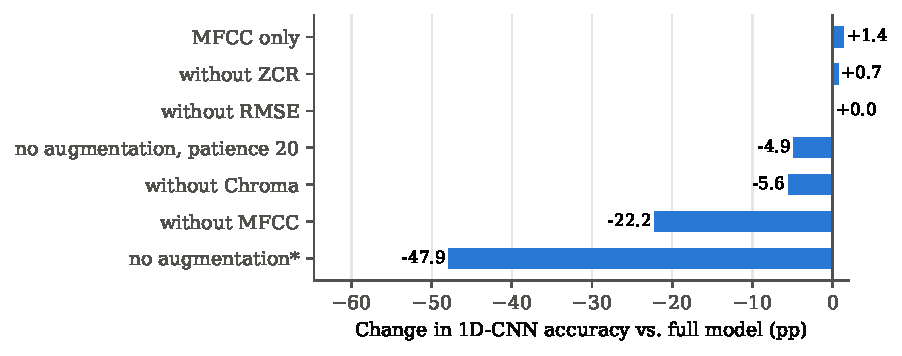
\includegraphics[width=\columnwidth]{../results/figures/fig_ablation.pdf}
\caption{Change in 1D-CNN accuracy when parts of the input are removed (paper-protocol split). *No augmentation
with the paper's early stopping, which halts before the model learns; see text.}
\label{fig:ablation}
\end{figure}
